\documentclass[sigconf]{acmart}

\usepackage{multicol}
\usepackage{multirow}
\usepackage{booktabs} % For formal tables
\usepackage[utf8]{inputenc}
\usepackage{algorithm,amsmath,lipsum,xcolor,caption}
\DeclareMathOperator{\sgn}{sign}
\DeclareCaptionFont{lightblue}{\color{blue}}
%\captionsetup[algorithm]{labelfont={bf,lightblue}, textfont={it}}
%\renewcommand{\thealgorithm}{\thechapter.\arabic{algorithm}}

\sloppy

% Copyright
%\setcopyright{none}
%\setcopyright{acmcopyright}
%\setcopyright{acmlicensed}
\setcopyright{rightsretained}
%\setcopyright{usgov}
%\setcopyright{usgovmixed}
%\setcopyright{cagov}
%\setcopyright{cagovmixed}


% DOI
%\acmDOI{}

% ISBN
%\acmISBN{123-4567-24-567/08/06}

%Conference
\acmConference[UFMG 2017]{Machine Learning Class}{June 2017}{Belo Horizonte, Minas Gerais, Brasil}
\acmYear{2017}
\copyrightyear{2017}



\begin{document}
\title{Machine Learning Boosting Algorithm:\\ A study case with Tic Tac Toe} 
%\titlenote{Produces the permission block, and copyright information}
\subtitle{Trabalho Prático 2}
%\subtitlenote{}



\author{Raphael Ottoni}
%\authornote{The secretary disavows any knowledge of this author's actions.}
\affiliation{%
 \institution{Universidade Federal de Minas Gerais}
 \streetaddress{}
 \city{Belo Horizonte} 
 \state{Minas Gerais} 
 \country{Brazil}
 \postcode{}
}
\email{rapha@dcc.ufmg.br}



% The default list of authors is too long for headers}
%\renewcommand{\shortauthors}{B. Trovato et al.}
%\renewcommand{\shortauthors}{}

%\begin{abstract}
%\end{abstract}

%
% The code below should be generated by the tool at
% http://dl.acm.org/ccs.cfm
% Please copy and paste the code instead of the example below. 
%
%\begin{CCSXML}
%<ccs2012>
% <concept>
%  <concept_id>10010520.10010553.10010562</concept_id>
%  <concept_desc>Computer systems organization~Embedded systems</concept_desc>
%  <concept_significance>500</concept_significance>
% </concept>
% <concept>
%  <concept_id>10010520.10010575.10010755</concept_id>
%  <concept_desc>Computer systems organization~Redundancy</concept_desc>
%  <concept_significance>300</concept_significance>
% </concept>
% <concept>
%  <concept_id>10010520.10010553.10010554</concept_id>
%  <concept_desc>Computer systems organization~Robotics</concept_desc>
%  <concept_significance>100</concept_significance>
% </concept>
% <concept>
%  <concept_id>10003033.10003083.10003095</concept_id>
%  <concept_desc>Networks~Network reliability</concept_desc>
%  <concept_significance>100</concept_significance>
% </concept>
%</ccs2012>  
%\end{CCSXML}

%\ccsdesc[500]{Computer systems organization~Embedded systems}
%\ccsdesc[300]{Computer systems organization~Redundancy}
%\ccsdesc{Computer systems organization~Robotics}
%\ccsdesc[100]{Networks~Network reliability}

\keywords{Machine Learning, boosting, Adaboost}

\maketitle

\input{Introducao}
%\input{adaboost}
\section{Dataset}\label{sec:dataset}

O \emph{dataset} utilizado neste experimento é o \emph{tic-tac-toe}, disponível em \url{https://archive.ics.uci.edu/ml/datasets/Tic-Tac-Toe+Endgame}. Cada linha desde \emph{dataset} representa um jogo da velha realizado e o label de qual jogador venceu aquela partida. Caso tenha sido o jogador "x" ele é positivo e se foi o jogador "o", este label é negativo. É interessante relatar, que nesta base da dados, não há exemplos de empate. Acredito que isto tenha sido feito propositalmente para que padecemos utilizar um classificador binário na classificação ao invés  de alguma outra técnica, por exemplo a \emph{one-against-all}. A tabela~\ref{tab:dataset} mostra a caracterização deste \emph{dataset}.

\begin{table}[h!]
\centering
\begin{tabular}{lc}
\textbf{Vencedor} & \textbf{Quantidade} \\ \hline 
x        & 626       \\
o        & 332       \\
total    & 958       \\
\end{tabular}
\caption{Tic-Tac-Toe Dataset}
\label{tab:dataset}
\end{table} 


Como dito antes, cada linha dos dados representa uma instância do jogo em que o jogador `x' ganhou ("positive") ou perder ("negative"). A figura~\ref{fig:representation} descreve com mais detalhe a representação de um jogo: um vetor de 10 posições, em que as primeiras nove são mapeadas diretamente para as 9 posições de um jogo da velha ( começando do canto superior esquerdo), seguido de um label mostrando se o jogador 'x' ganhou ou perdeu. Cada uma das 9 primeiras posições contem um dos três valores possíveis: 'b' para blank, 'x' para o primeiro jogador e 'o' para o segundo.   

\begin{figure}[h]
  
\includegraphics[width=\linewidth]{imgs/game_representation.png}
  \caption{Representação de um jogo.}
  \label{fig:representation}
\end{figure}

\input{Implementacao}
\section{Análise}
Todas as analises foram feitas baseadas em calculo de erro simples e utilizando o algoritmo de validação cruzada com 5 partições. Nestas análises não foram variadas o número de partições por acreditar que este trabalho prático é voltado para o algoritmo de \emph{boosting} e não de validação cruzada. Em todos os gráficos a seguir, o erro apresentando é a dado como a media do erro encontrado em cada validação cruzada.


A primeira análise interessante a ser feita é a relação dos errors tanto de treino quanto de validação com o número de iterações do \emph{Aadaboost}. Lembrando que o número de iterações é o número de classificadores fracos que queremos utilizar.

\begin{figure}[h]
  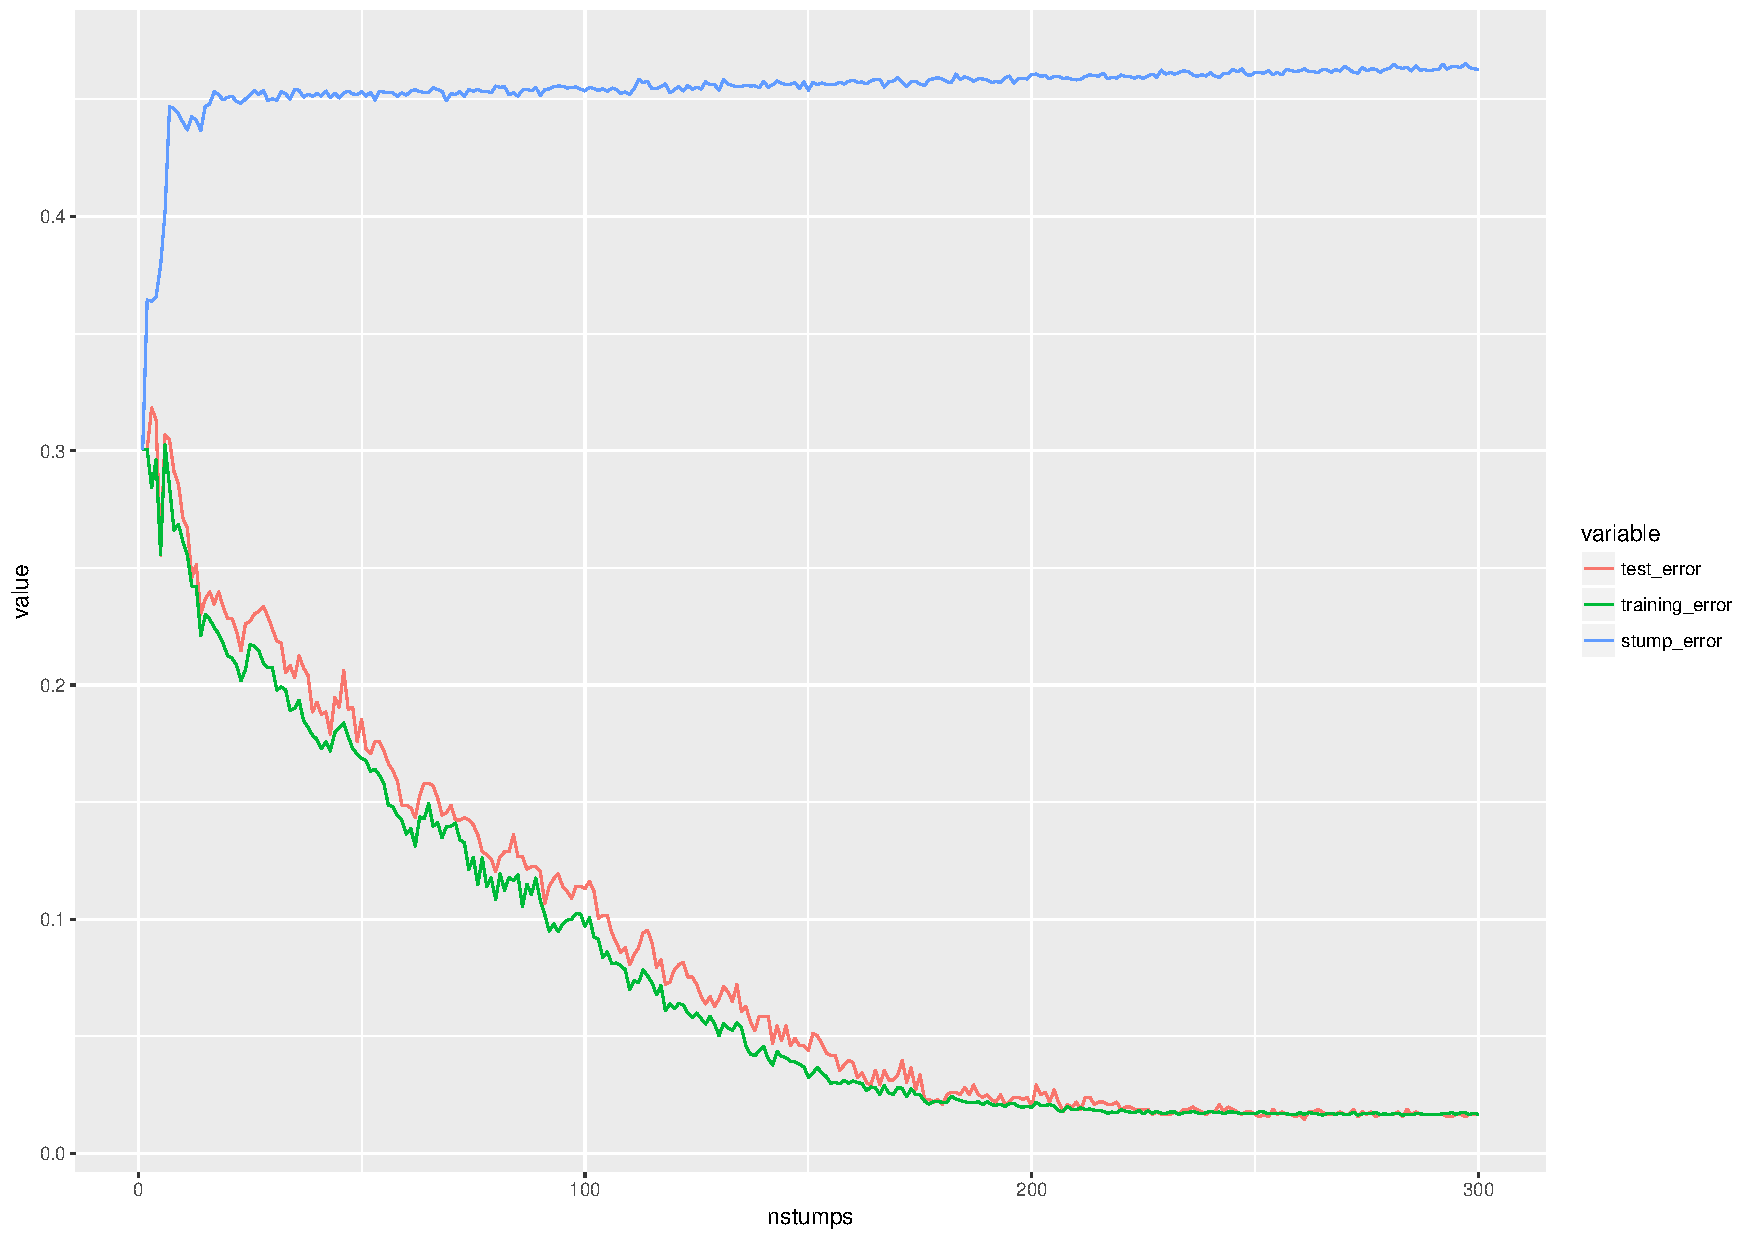
\includegraphics[width=\linewidth]{imgs/accuracy.pdf}
  \caption{Adaboost erros por quantidade de \emph{weak classifiers}}
  \label{fig:adaboostAccuracy}
\end{figure}

Como pode ser visto na Figura.~\ref{fig:adaboostAccuracy}, como esperado os errors de treino e de teste tendem a cair com o aumento de stumps escolhidos. Demonstrando assim a força da combinação de classificadores fracos, podemos ver que ambos convergem para um valor próximo de 0.02 tendo o erro de validação maior que o erro de treino durante a convergência. É interessante realçar que mesmo com uma grande escolha de um número grande de stumps, cerca de 6 vezes mais do que os stumps disponíveis, o \emph{Adaboost} não sofreu de \emph{overfit} e convergiu.

Outra padrão esperado que foi mostrado neste gráfico é o aumento do erro de cada stump escolhido (em cada uma das iterações) e sua convergência para um valor próximo de 0.5, mostrando assim, que idealmente, classificadores interessantes para o \emph{Adaboost} são aqueles um pouco melhores que o aleatório (0.5). 

Podemos ver também, que o primeiro stump escolhido já e responsável por aproximadamente 0.7 de acurácia (erro de 0.3 quando todas as observações tem a mesma importância), isso provavelmente deve ser fruto do desbalanceamento de classes, quase o dobro de partidas no dataset foram vencidas pelo jogador "x" (Tabela~\ref{tab:dataset}). Se olharmos com mais detalhes as Figuras~[\ref{fig:main2_2},\ref{fig:main_2_5}] veremos que o primeiro stump escolhido é o de identificação 27, que se consultarmos a Tabela~\ref{tab:stumps}, vemos que é o caso quando o jogador 'o' marcou na posição central do jogo da velha. O que faz sentido se pensarmos na estratégia ótima do jogo da velha. Este jogo é conhecido por ser desbalanceado de modo que quem começa se adotar a estratégia ótima não poderá perder, Se entrar em detalhes, tal estratégia envolve nunca preencher o quadrado central. 

\begin{figure}[h]
  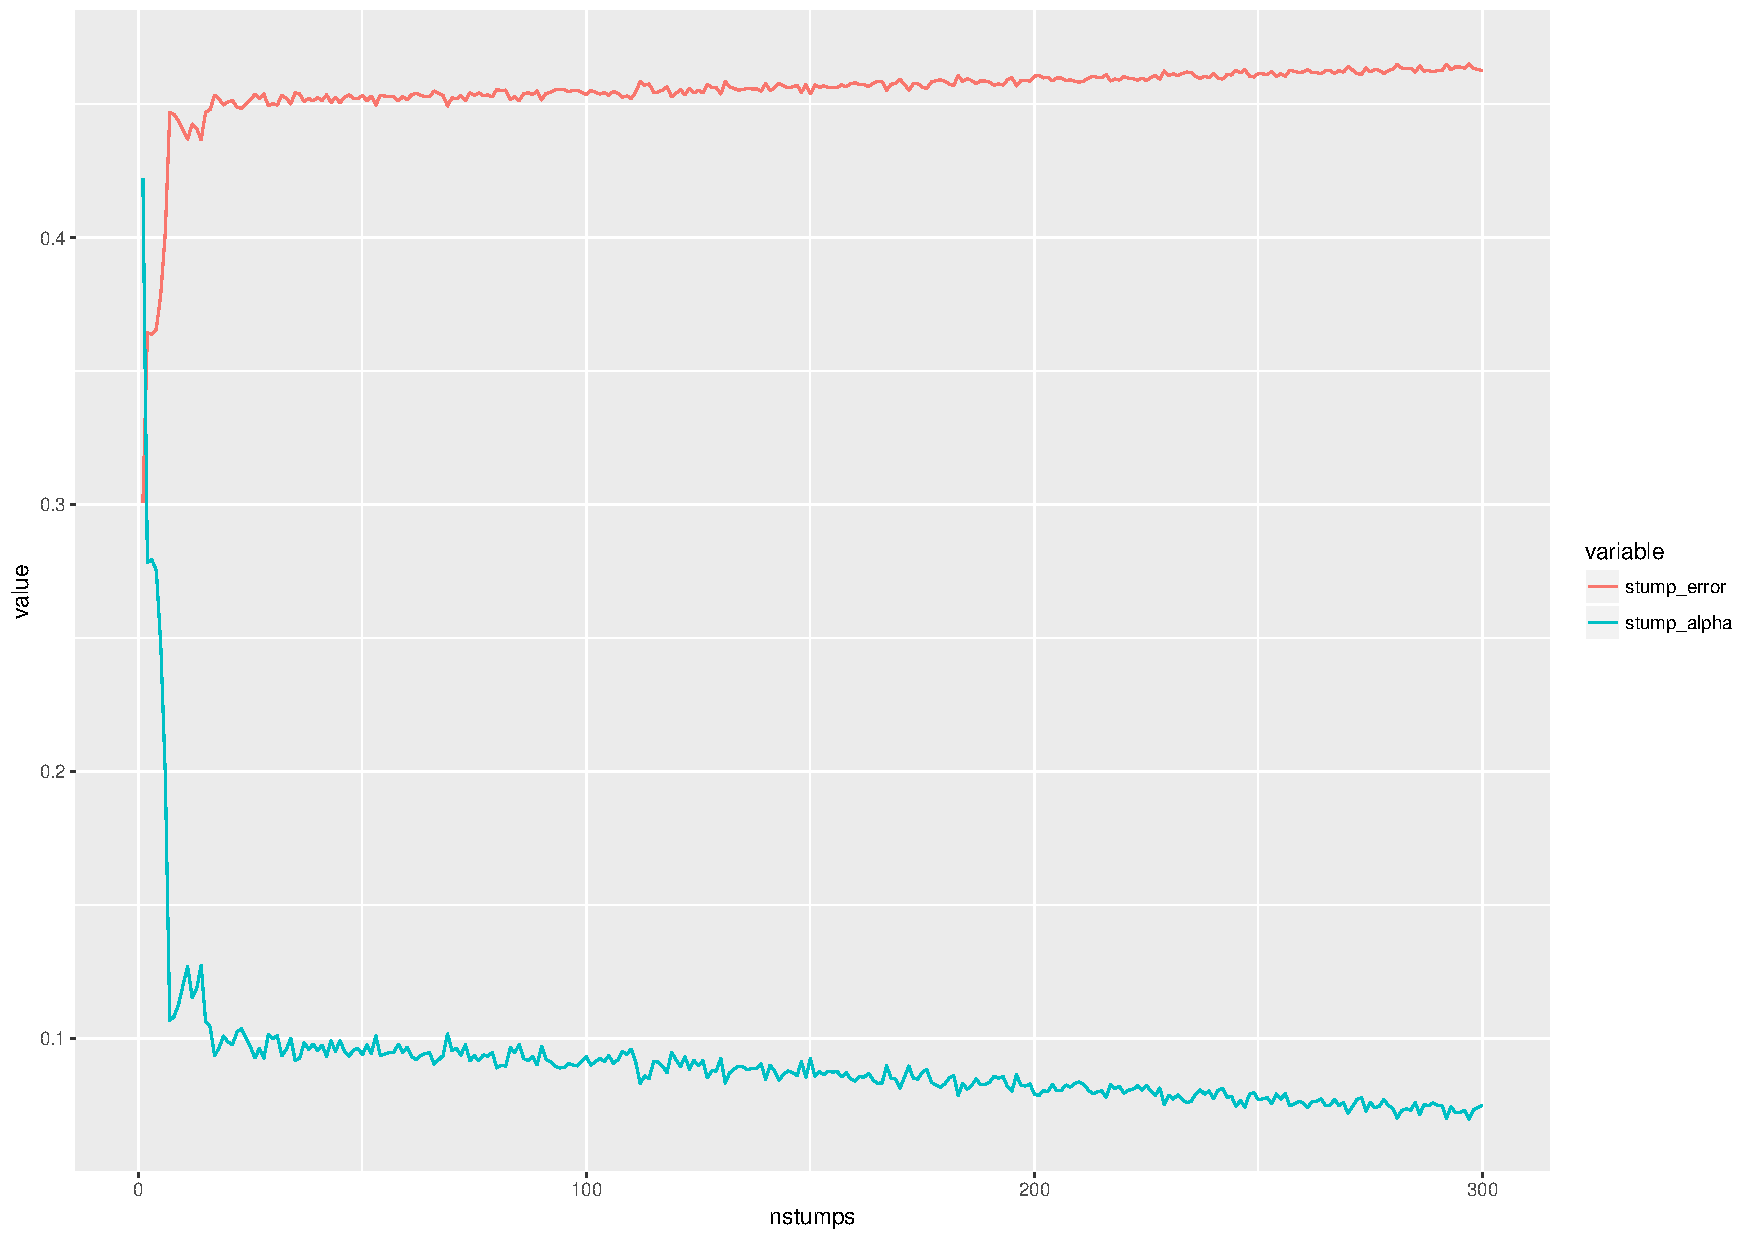
\includegraphics[width=\linewidth]{imgs/alpha_error.pdf}
  \caption{Adaboost \emph{stumps} escolhidos em cada iteração com seus  alphas e errors  associados}
  \label{fig:adaboost_alphas}
\end{figure}

Outra análise interessante é relação dos alphas e dos errors de cada stump escolhido (Pseudocódigo.~\ref{pseudocode:adaboost}, calculo $\alpha_m$), por definição matemática o alpha  e erro do stump estão inversamente relacionados: quem erra mais tem um alpha menor e consecutivamente contribui menos para a classificação final. Como podemos ver pela Figura.~\ref{fig:adaboost_alphas}, os primeiros stumps tendem a ser escolhidos com uma importância (alpha) mais alta e subsecutivamente essas importâncias tendem a decrescer suavemente fazendo com que a importância dos últimos stumps escolhidos sejam aproximadamente iguais. Porem como o \emph{Adaboost} atualiza os pesos de forma que o próximo stump é enviesado para escolher aquele que acerta mais os que o anterior errou, na \emph{big-picture}, mesmo tendo importância próxima eles tendem a contribuir com pouca interseção, são especialistas em partes diferentes dos dados.

%\input{related_works}
\section{Discussão e Conclusão}
Este trabalho prático foi interessante pois pude ver na prática a ideia de que se pode criar um classificador forte a partir de classificadores fracos. Mais do que isso, a técnica utilizada, \emph{Adaboost}, se provou muito resistente a  \emph{overfitting} e pode ser utilizada com qualquer tipo de classificadores. Não sendo limitada apenas a \emph{stumps}, como foi feito neste trabalho prático. 

Outra parte importante deste trabalho, foi comprovar conceitos sobre boosting aprendidos em sala de aula, como o porque é interessante apenas utilizar classificadores fracos no \emph{ensamble} e o porque idealmente eles deveriam ser um pouco melhores do que um classificador aleatório.


%\bibliographystyle{ACM-Reference-Format}
%\bibliography{bibliography} 

\end{document}
